\documentclass{article}
\usepackage{tikz}
\usepackage{tkz-euclide}
\usetikzlibrary{arrows}
\begin{document}


\section{Draw lines}


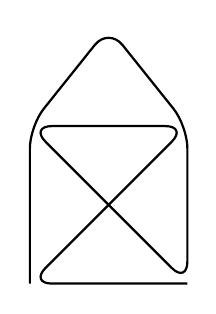
\begin{tikzpicture}
\tikz \draw[thick,rounded corners=8pt]
(0,0) -- (0,2) -- (1,3.25) -- (2,2) -- (2,0) -- (0,2) -- (2,2) -- (0,0) --
(2,0);
\end{tikzpicture}



We are working on
\tikz    \draw (-1.5, 0) -- (1.5, 0);


\section{Curved Lines}


Curved line
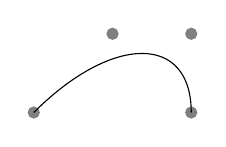
\begin{tikzpicture}
    \filldraw [gray] (0,0) circle [radius=2pt]
    (1,1) circle [radius=2pt] (2,1) circle [radius=2pt] (2,0) circle
    [radius=2pt];
      \draw (0,0) .. controls (1,1) and (2,1) .. (2,0);
  \end{tikzpicture}

\section{Circle}


Circle: \tikz \draw (0,0) circle [radius=10pt];

\bigskip

Ellipse: \tikz \draw (0,0) ellipse [x radius=20pt, y radius=10pt];

\bigskip

Another circle: 
\begin{tikzpicture}
    \draw (-1.5,0) -- (1.5,0);
    \draw (0,-1.5) -- (0,1.5);
    \draw (0,0) circle [radius=1cm];
\end{tikzpicture}


\bigskip

Add rectangle:

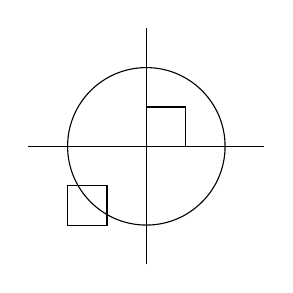
\begin{tikzpicture}
\draw (-1.5,0) -- (1.5,0);
\draw (0,-1.5) -- (0,1.5);
\draw (0,0) circle [radius=1cm]; \draw (0,0) rectangle (0.5,0.5); \draw
(-0.5,-0.5) rectangle (-1,-1);
\end{tikzpicture}


\bigskip

\section{Grid lines}


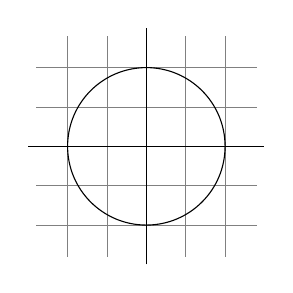
\begin{tikzpicture}
    \draw[step=.5cm,gray,very thin] (-1.4,-1.4) grid (1.4,1.4); \draw (-1.5,0)
    -- (1.5,0);
    \draw (0,-1.5) -- (0,1.5);
    \draw (0,0) circle [radius=1cm];
\end{tikzpicture}


\bigskip

Define style:

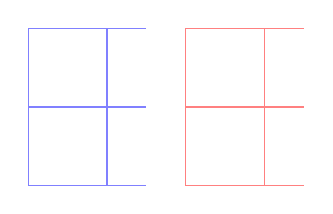
\begin{tikzpicture}
    [Karl’s grid/.style ={help lines,color=#1!50},
    Karl’s grid/.default=blue]
   \draw[Karl’s grid]     (0,0) grid (1.5,2);
   \draw[Karl’s grid=red] (2,0) grid (3.5,2);
  
\end{tikzpicture}



\section{Arc}

\begin{tikzpicture}[scale=3]
    \draw[step=.5cm,gray,very thin] (-1.4,-1.4) grid (1.4,1.4); \draw (-1.5,0)
    -- (1.5,0);
    \draw (0,-1.5) -- (0,1.5);
    \draw (0,0) circle [radius=1cm];
    \draw (3mm,0mm) arc [start angle=0, end angle=30, radius=3mm];
\end{tikzpicture}


\bigskip

Fill arc with color, plus clipping:
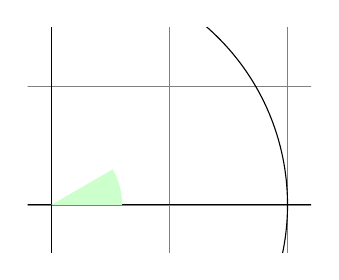
\begin{tikzpicture}[scale=3]
    \clip (-0.1,-0.2) rectangle (1.1,0.75); \draw[step=.5cm,gray,very thin]
    (-1.4,-1.4) grid (1.4,1.4); \draw (-1.5,0) -- (1.5,0);
    \draw (0,-1.5) -- (0,1.5);
    \draw (0,0) circle [radius=1cm];
    \fill[green!20!white] (0,0) -- (3mm,0mm)
arc [start angle=0, end angle=30, radius=3mm] -- (0,0); \end{tikzpicture}


\section{Use coordinate}

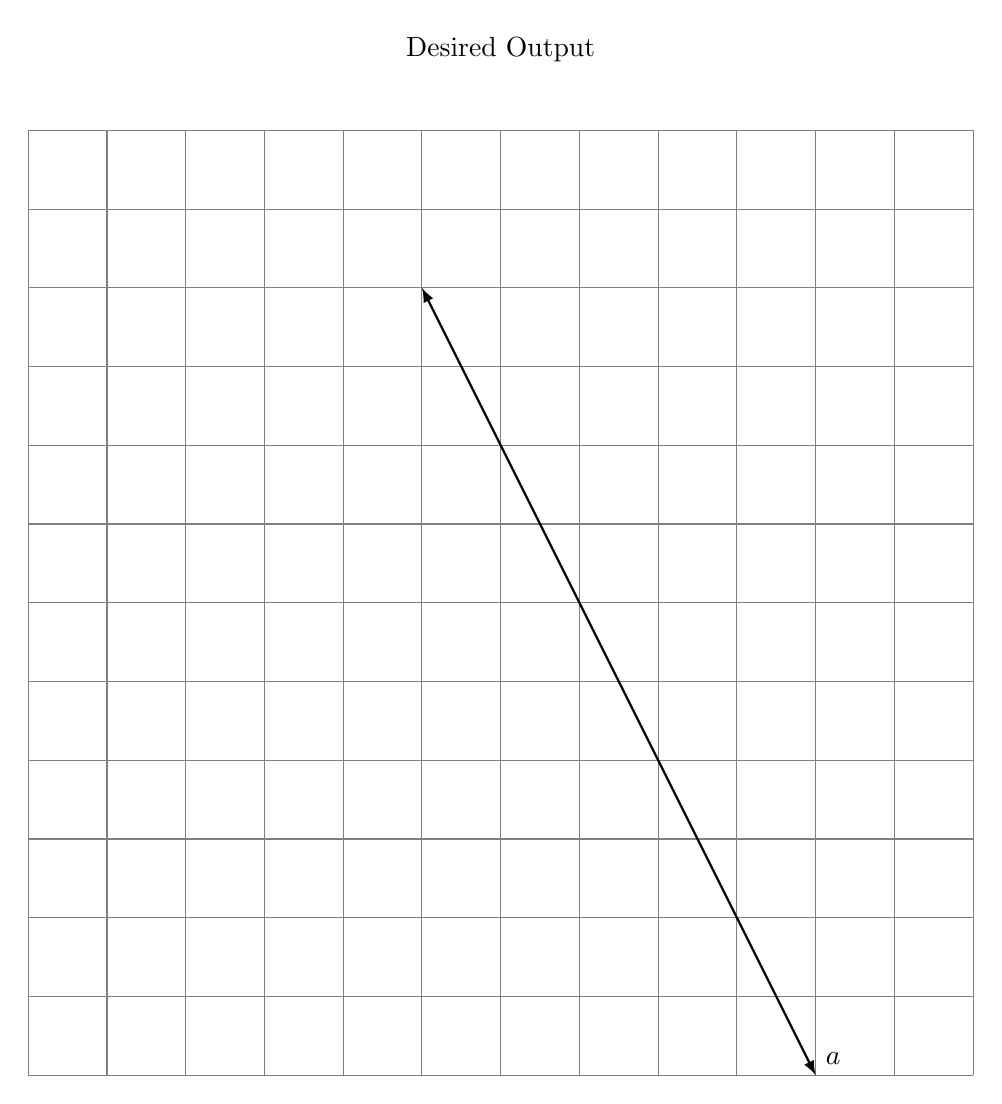
\begin{tikzpicture}
   \tkzInit[xmax=6,ymax=6,xmin=-6,ymin=-6]
   \tkzGrid
   \tkzAxeXY
   \draw[ thick,latex-latex] (-1,4) -- (4,-6)
   node[anchor=south west] {$a$}; % two points for drawing
   2x+y=2
   \tkzText[above](0,6.75){Desired Output}
\end{tikzpicture}

\section{Foreach}


\bigskip

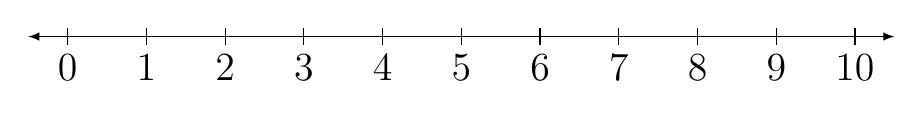
\begin{tikzpicture}
    % draw arrow line
    \draw[latex-latex] (-0.5,0) -- (10.5, 0);
    % draw vertical bar
    \foreach \x in {0, 1, ..., 10}
        \draw[shift={(\x,0)}, color=black] (0pt, 3pt) -- (0pt, -3pt);
    % draw number
    \foreach \x in {0, 1, ..., 10}
        \draw[shift={(\x,0)}, color=black] (0pt, 0pt) -- (0pt, -3pt)
        node[below] {{\Large $\x$}};

\end{tikzpicture}

Divide $(0, 1)$ into 10 segments \bigskip

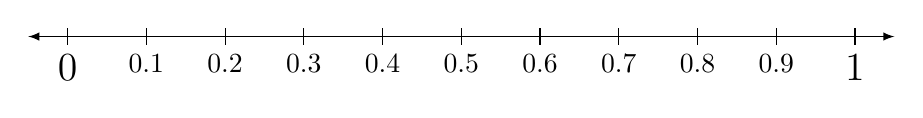
\begin{tikzpicture}
    % draw arrow line
    \draw[latex-latex] (-0.5,0) -- (10.5, 0);
    % draw vertical bar
    \foreach \x in {0, 1, ..., 10}
        \draw[shift={(\x,0)}, color=black] (0pt, 3pt) -- (0pt, -3pt);

    \draw[color=black] (0pt, 0pt) -- (0pt, -3pt) 
            node[below] {\Large $0$};
    
    \draw[shift={(10,0)}, color=black] (0pt, 0pt) -- (0pt, -3pt)
            node[below] {\Large $1$};

    \foreach \x in {1,2, ..., 9}
        \draw[shift={(\x,0)}, color=black] (0pt, 0pt) -- (0pt, -3pt)
            node[below] {$0.\x$};
\end{tikzpicture}

Divide $(0.0, 1.0)$ into 10 segments \bigskip

\end{document}

